\section{Jet Classification}
{{\footnotesize
\begin{description}[labelwidth=5em, labelsep=1em, leftmargin=*, align=left, itemsep=0.3em, parsep=0em]
  \item[date:] 2024-05-01
  \item[last\_updated:] 2024-05
  \item[expired:] unkown
  \item[valid:] yes
  \item[url:] \href{https://github.com/fastmachinelearning/fastml-science/tree/main/jet-classify}{https://github.com/fastmachinelearning/fastml-science/tree/main/jet-classify}
  \item[domain:] Particle Physics
  \item[focus:] Real-time classification of particle jets using HL-LHC simulation features
  \item[keywords:]
    - classification
    - real-time ML
    - jet tagging
    - QKeras
  \item[task\_types:]
    - Classification
  \item[ai\_capability\_measured:]
    - Real-time inference
    - model compression performance
  \item[metrics:]
    - Accuracy
    - AUC
  \item[models:]
    - Keras DNN
    - QKeras quantized DNN
  \item[ml\_motif:]
    - Real-time
  \item[type:] Benchmark
  \item[ml\_task:] Supervised Learning
  \item[notes:] Includes both float and quantized models using QKeras
  \item[contact.name:] Jules Muhizi
  \item[contact.email:] unkown
  \item[dataset.name:] JetClass
  \item[dataset.url:] \href{https://zenodo.org/record/6619768}{https://zenodo.org/record/6619768}
  \item[results.name:] ChatGPT LLM
  \item[results.url:] \href{https://docs.google.com/document/d/1runrcij-eoH3\_lgGZ8wm2z1YbL1Qf5cSNbVbHyWFDs4}{https://docs.google.com/document/d/1runrcij-eoH3\_lgGZ8wm2z1YbL1Qf5cSNbVbHyWFDs4}
  \item[fair.reproducible:] True
  \item[fair.benchmark\_ready:] True
  \item[ratings.software.rating:] 0
  \item[ratings.software.reason:] Not analyzed.
  \item[ratings.specification.rating:] 9.0
  \item[ratings.specification.reason:] Task and format (multiple-choice QA with 5 options) are clearly defined; grounded in ConceptNet with consistent structure, though no hardware/system constraints are specified.
  \item[ratings.dataset.rating:] 9.0
  \item[ratings.dataset.reason:] Public, versioned, and FAIR-compliant; includes metadata, splits, and licensing; well-integrated with HuggingFace and other ML libraries.
  \item[ratings.metrics.rating:] 9.0
  \item[ratings.metrics.reason:] Accuracy is a simple, reproducible metric aligned with task goals; no ambiguity in evaluation.
  \item[ratings.reference\_solution.rating:] 8.0
  \item[ratings.reference\_solution.reason:] Several baseline models (e.g., BERT, RoBERTa) are reported with scores; implementations exist in public repos, but not bundled as an official starter kit.
  \item[ratings.documentation.rating:] 7.0
  \item[ratings.documentation.reason:] Clear paper, GitHub repo, and integration with HuggingFace Datasets; full reproducibility requires manually connecting models to dataset.
  \item[id:] jet\_classification
  \item[Citations:] \cite{duarte2022fastml}
  \item[Ratings:]
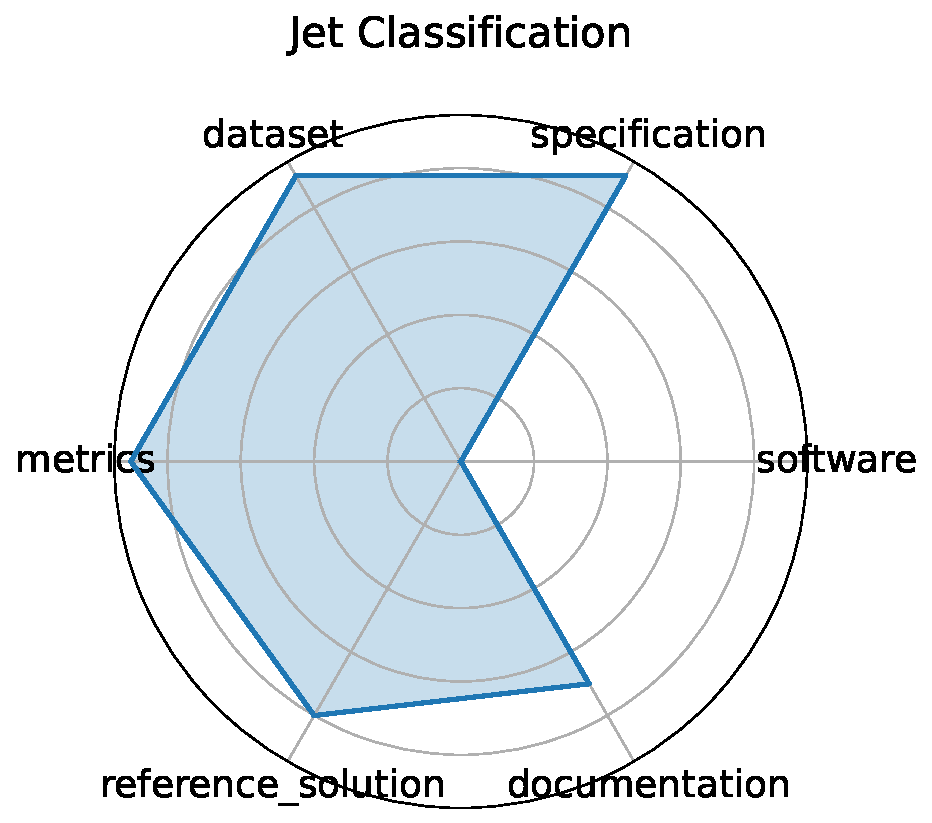
\includegraphics[width=0.2\textwidth]{jet_classification_radar.pdf}
\end{description}
}}
\clearpage